\documentclass[a4paper,14pt]{report}
\usepackage[T2A]{fontenc}
\usepackage[utf8]{inputenc}
\usepackage[english,russian]{babel}
\usepackage{listings}
\usepackage{geometry}
\usepackage{amssymb}
\usepackage{amsmath}
\usepackage[14pt]{extsizes}
\geometry{left=2cm}
\geometry{right=1.5cm}
\geometry{top=1cm}
\geometry{bottom=2cm}
\pagestyle{plain}
\usepackage{pgfplots}
\usepackage{filecontents}
\usepackage{graphicx}
\usepackage{indentfirst}
\DeclareGraphicsExtensions{.png}
\graphicspath{{images/}}
\usetikzlibrary{datavisualization}
\usetikzlibrary{datavisualization.formats.functions}
\usepackage{tabularx}
\pgfplotsset{width=7 cm}

\usepackage{tocloft}

\renewcommand\cftchapdotsep{\cftdot}
\renewcommand\cftsecdotsep{\cftdot}
\renewcommand{\cftchapleader}{\cftdotfill{\cftchapdotsep}}


\begin{filecontents}{thread1.dat}
	0 0
	10 1.409
	20 2.813
	30 4.221
	40 5.629
	50 7.036
\end{filecontents}

\begin{filecontents}{thread3.dat}
	0 0
	10 0.773
	20 1.482
	30 2.174
	40 2.878
	50 3.579
\end{filecontents}

% Для листинга кода:
\lstset{ %
language=c++,                 % выбор языка для подсветки
basicstyle=\small\sffamily, % размер и начертание шрифта для подсветки кода
numbers=left,               % где поставить нумерацию строк (слева\справа)
numberstyle=\tiny,           % размер шрифта для номеров строк
stepnumber=1,                   % размер шага между двумя номерами строк
numbersep=5pt,                % как далеко отстоят номера строк от подсвечиваемого кода
showspaces=false,            % показывать или нет пробелы специальными отступами
showstringspaces=false,      % показывать или нет пробелы в строках
showtabs=false,             % показывать или нет табуляцию в строках
frame=single,              % рисовать рамку вокруг кода
tabsize=4,                 % размер табуляции по умолчанию равен 2 пробелам
captionpos=t,              % позиция заголовка вверху [t] или внизу [b]
breaklines=true,           % автоматически переносить строки (да\нет)
breakatwhitespace=false, % переносить строки только если есть пробел
escapeinside={\#*}{*)}   % если нужно добавить комментарии в коде
}

% Для измененных титулов глав:
\usepackage{titlesec, blindtext, color} % подключаем нужные пакеты
\definecolor{gray75}{gray}{0.75} % определяем цвет
\newcommand{\hsp}{\hspace{20pt}} % длина линии в 20pt
% titleformat определяет стиль
\titleformat{\chapter}[hang]{\Huge\bfseries}{\thechapter\hsp\textcolor{gray75}{|}\hsp}{0pt}{\Huge\bfseries}



\begin{document}
\begin{titlepage}
	\centering
	{\scshape\LARGE МГТУ им. Баумана \par}
	\vspace{3cm}
	{\scshape\Large Лабораторная работа №6\par}
	\vspace{0.5cm}
	{\scshape\Large По курсу: "Анализ алгоритмов"\par}
	\vspace{1.5cm}
	{\huge\bfseries Муравьиные алгоритмы\par}
	\vspace{2cm}
	\Large Работу выполнила: Овчинникова Анастасия, ИУ7-55Б\par
	\vspace{0.5cm}
	\LargeПреподаватели:  Волкова Л.Л., Строганов Ю.В.\par

	\vfill
	\large \textit {Москва, 2019} \par
\end{titlepage}

\tableofcontents

\newpage
\chapter*{Введение}
\addcontentsline{toc}{chapter}{Введение}
Целью данной лабораторной работы является приобритение навыка параметризации метода на примере решения задачи коммивояжера методом, основанным на муравьином алгоритме.

Задачи лабораторной работы:

\begin{enumerate}
	\item параметризация - выбор таких параметров или их сочетаний метода, при которых этот метод решает класс задач с наилучшим качеством;
	\item провести сравнительный анализ эвристического метода и метода полного перебора;
	\item минимизировать разницу между муравьиным алгоритмом и полным перебором.
\end{enumerate}


\chapter*{Аналитическая часть}
\addcontentsline{toc}{chapter}{Аналитическая часть}

Задача коммивояжёра (или TSP от англ. Travelling salesman problem) — одна из самых известных задач комбинаторной оптимизации, заключающаяся в поиске самого выгодного маршрута, проходящего через указанные города хотя бы по одному разу с последующим возвратом в исходный город.

Сама  задача  формулируется  довольно  просто:  имеется n городов, расстояния между которыми нам известны. Коммивояжер находится в одном из этих городов, и желает объехать все города, при этом посетив каждый из них  ровно  один  раз, а  затем вернуться  в  исходный  город. Кроме  того, искомый путь должен иметь наименьшую длину.

Расстояния между городами обычно задаются с помощью матрицы смежности.
Задача  коммивояжера  является NP-трудной,  даже  когда матрица расстояний между городами симметрична, то есть задача коммивояжера не может быть проверена за полиномиальное время, однако задача разрешения для задачи коммивояжера принадлежит к классу NP-полных задач.

В данной лабораторной работе рассматривается случай, когда из любого города можно попасть в любой город и все дороги(маршруты) являются неориентированными (то есть рассматривается полный граф и симметричная матрица смежности).

\section*{Алгоритмы решения задачи коммивояжёра}
\addcontentsline{toc}{section}{Алгоритмы решения задачи коммивояжёра}

Существует множество различных способов решения этой задачи, как точных, так и приближенных. В качестве примера точного метода ее решения можно  привести  полный  перебор  — перебор  всевозможных вариантов и в выбор среди них оптимального. Все  алгоритмы,  сокращающие  полный  перебор,  не  дают  точного значения. С их помощью можно найти только приближённое решение задачи, при этом не гарантируется, что погрешность вычислений будет низка.

\subsection*{Полный перебор}
\addcontentsline{toc}{section}{Полный перебор}

Алгоритм  полного перебора  (также  известен  как  метод  грубой  силы) осуществляет  поиск  всех  решений  путём  перебора  всех  вариантов  в количестве N! штук, позволяя получить точное решение задачи. Однако как уже было сказано, задача коммивояжёра относится к классу NP-трудных: уже при относительно небольшом числе городов (66 и более) она не может быть решена методом перебора вариантов никакими теоретически мыслимыми компьютерами за время, меньшее нескольких миллиардов лет.

\subsection*{Муравьиный алгоритм}
\addcontentsline{toc}{section}{Муравьиный алгоритм}

В основе муравьиного алгоритма лежат принципы самоорганизации муравьиной колонии.

Идея   муравьиного   алгоритма   заключается в   моделировании поведения  муравьев,  связанного  с  их  способностью  находить  кратчайший путь от муравейника к источнику пищи и адаптироваться к изменяющимся условиям,  находя  новый  кратчайший  путь.  При  своем  движении  муравей метит  свой  путь  феромоном,  и  эта  информация  используется  другими муравьями.  Это  и  является  главным  правилом  поведения  каждого  из представителей  колониив  случае,  если  старый  маршрут  стал  недоступен.

Рассмотрим  случай, когда  на  оптимальном пути возникает преграда. В этом случае необходимо определение нового оптимального пути. Дойдя до преграды, муравьи с равной вероятностью будут обходить её справа и слева.  То же самое будет происходить и на обратной стороне преграды. Однако, те муравьи, которые случайно выберут кратчайший путь,  будут быстрее его проходить,  и за несколько передвижений он будет более  обогащён  феромоном.   Поскольку  движение  муравьёв  определяется концентрацией феромона, то следующие будут предпочитать именно этот путь, продолжая обогащать его феромоном до тех пор, пока этот путь по какой-либо причине не станет недоступен.

Испарение феромона в воздухе гарантирует, что найденное решение не будет единственным, и муравьи будут продолжать искать и другие пути. Если мы моделируем  процесс  такого  поведения  на  графе,  ребра  которого — всевозможные  пути  движения,  то  в  течение  некоторого  времени  наиболее обогащенный феромоном путь и будет наикратчайшим, что и даст решение задачи.

Преимуществами   алгоритма   являются   невысокая   погрешность найденного  решения,  низкие  временные  затраты  при  работе  с  графами большой  размерности,  модифицируемость  алгоритма  и  возможность распараллеливания.

\subsection*{Применение муравьиного алгоритма}
\addcontentsline{toc}{section}{Применение муравьиного алгоритма}

Любой муравьиный алгоритм, независимо от модификаций, представим вследующем виде.
\begin{enumerate}
	\item Инициализация параметров.
\end{enumerate}
Пока (условия выхода не выполнены):
\begin{enumerate}
	\item создаём Муравьёв;
	\item поиск решений;
	\item обновление феромона.
\end{enumerate}

Пусть имеется M городов и задана симметричная матрица смежности $D[M x M]$.
Рассмотрим каждый шаг в цикле более подробно.

\subsubsection*{Инициализация параметров}
\addcontentsline{toc}{section}{Инициализация параметров}

На  этом  этапе  задаётся  начальный  уровень  феромона.    Онинициализируется  небольшим  положительным  числом  для  того,  чтобы  наначальном  шаге  вероятности  перехода  в  следующую  вершину  не  былинулевыми. Кроме начального уровня феромонов необходимо также задать следующие параметры.
\begin{enumerate}
	\item $\alpha$ - параметр влияния длины пути.
	\item $\beta$ - параметр влияния феромона ($\alpha$ + $\beta$ = const).
	\item $\rho$ $\in$ (0, 1) - коэффицент испарения феромона.
	\item $t_{max}$ - количество поколений муравьёв (количество итераций в алгоритме).
	\item $\tau_{min}$ - минимальное возможное значение феромона. Феромон не должен падать ниже этой константы и обнуляться, чтобы не обнулялась вероятность (см. ниже).
	\item $\tau_{start}$ - начальное значение феромона.
	\item $Q$ - количество феромона, переносимого муравьем.
\end{enumerate}

\subsubsection*{Создание муравьёв}
\addcontentsline{toc}{section}{Создание муравьёв}

В каждый город помещается по муравью (количество муравьев равно количеству городов).

\subsubsection*{Поиск решений}
\addcontentsline{toc}{section}{Поиск решений}

Каждый муравей хранит в памяти список пройденных им узлов. Этот список называют списком запретов (tabu list) или просто памятью муравья. Выбирая узел для следующего шага, муравей «помнит» об уже пройденных узлах и не рассматривает их в качестве возможных для перехода. На каждом шаге список запретов пополняется новым узлом, а перед новой итерацией алгоритма – то есть перед тем, как муравей вновь проходит путь – он опустошается.

Кроме списка запретов, при выборе узла для перехода муравей руководствуется «привлекательностью» ребер, которые он может пройти. Она зависит, во-первых, от расстояния между узлами (то есть от веса ребра), а во-вторых, от следов феромонов, оставленных на ребре прошедшими по нему ранее муравьями. Естественно, что в отличие от весов ребер, которые являются константными, следы феромонов обновляются на каждой итерации алгоритма: как и в природе, со временем следы испаряются, а проходящие муравьи, напротив, усиливают их.

Пусть k-й муравей находится в i-м городе. Тогда вероятность посещения города j, который ранее на данной итерации муравьем не посещался, будет вычисляться по следующей формуле.

\begin{equation}\label{form:way}
 p_{i,j}={\frac {(\tau _{i,j}^{\alpha })(\eta _{i,j}^{\beta })}{\sum (\tau _{i,j}^{\alpha })(\eta _{i,j}^{\beta })}}
 \end{equation}
 \begin{align*}
    \text{где} \\
   \tau _{i,j} &- \text{расстояние от города i до j;} \\
    \eta _{i,j} = \frac{1}{D_{ij}} &- \text{привлекательность города для муравья;} \\
    \alpha &- \text{параметр влияния длины пути;} \\
    \beta &- \text{параметр влияния феромона.}
\end{align*}

Очевидно, что при $\beta$ = 0 алгоритм превращается в классический жадный алгоритм. Выбор правильного соотношения параметров является предметом исследований, и в общем случае производится на основании опыта.

\subsubsection*{Обновление феромона}
\addcontentsline{toc}{section}{Обновление феромона}

После того, как муравей успешно проходит маршрут, он оставляет на всех пройденных ребрах след, обратно пропорциональный длине пройденного пути:
\begin{equation}\label{form:eva}
    \tau _{ij}(t + 1)=(1-\rho )\tau _{ij}(t) + \sum\limits_{k=1}^n \Delta \tau _{k, ij}(t),
\end{equation}
\begin{align*}
    \text{где} \\
    \rho _{ij} &- \text{коэффицент испарения феромона ($	\rho$ $\in$ (0, 1));} \\
    \tau _{ij} &- \text{количество феромона на дуге ij;} \\
    \Delta \tau _{ij}(t) &- \text{количество отложенного феромона на данном шаге по времени.}
\end{align*}
Количество отложенного феромона на данном шаге по времени, обычно определяется следующим образом.
\begin{equation}\label{form:add}
    {\displaystyle \Delta \tau _{k, ij}(t)={\begin{cases} \frac{Q}{L_{k}}(t) & {\mbox{, если k-ый мурваей прошел по ребру ij}}\\0&{\mbox{, иначе}}\end{cases}}}
\end{equation}
\begin{align*}
    \text{где} \\
    Q &- \text{количество феромона, переносимого муравьем;} \\
    L_{k}(t) &- \text{длина сформ. маршрута k-го муравья на данном шаге по времени.}
\end{align*}


\chapter*{Конструкторская часть}
\addcontentsline{toc}{chapter}{Конструкторская часть}

В данном разделе будут описаны принципы работы выбранных решений и их блоксхемы.

\section*{Требования к программе}
\addcontentsline{toc}{section}{Требования к программе}

\textbf{Требования к вводу:}\\
На вход программе подается файл с содержанием следующего формата.
\begin{enumerate}
	\item В первой строке записано количетство городов (M).
	\item На каждой из последующих строк записаны строки матрицы смежности размерности M x M.
	\item Матрица симметричная.
	\item На главной диагонали матрицы записаны нули.
	\item Матрица смежности содержит целочисленные значения.
	\item Никаких других лишниих символов в файле содержаться не должно.
\end{enumerate}

Требования 2-4 являются следствием ограничений, накладываемых на граф. Эти ограничения обсуждались в аналитической части.

\textbf{Требования к программе:}\\
Программа должна решать задачу коммивояжёра и выводить длину оптимального (в случае муравьиного алгоритма) или самого короткого (в случае полного перебора) маршрута.

\section*{Схемы алгоритмов}
\addcontentsline{toc}{section}{Схемы алгоритмов}

Схема алгоритма полного перебора представлена на рисунке 1.
Схема метода createAdjacencyList(), используемого в алгоритме полного перебора, представлена на рисунке 2. Метод createAdjacencyList() из исходной матрицы смежности строит список смежжности. Это делается для того, чтобы можно было более удобно реализовать полный перебор.
Схема метода allPaths(), используемого в алгоритме полного перебора, представлена на рисунках 3-4. Схема метода isIn(), используемого в методе allPaths(), приведена на рисунке 5.

Обратим внимание, что в методах используется контейнер vector из стандартной библиотеки C++ и его методы. За более подробной информацией об этом контейнере и его методах следует обратиться к документации.

\begin{figure}[h]
\center{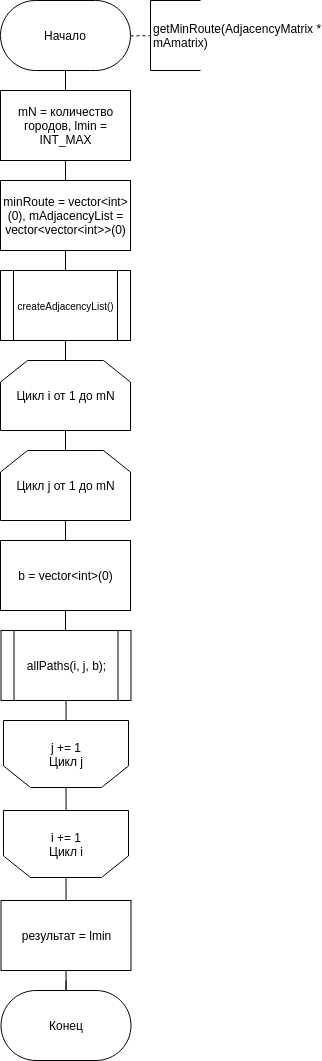
\includegraphics[height=19cm]{bforce}}
\caption{Схема алгоритма полного перебора}
\label{fig:image}
\end{figure}

\begin{figure}
\center{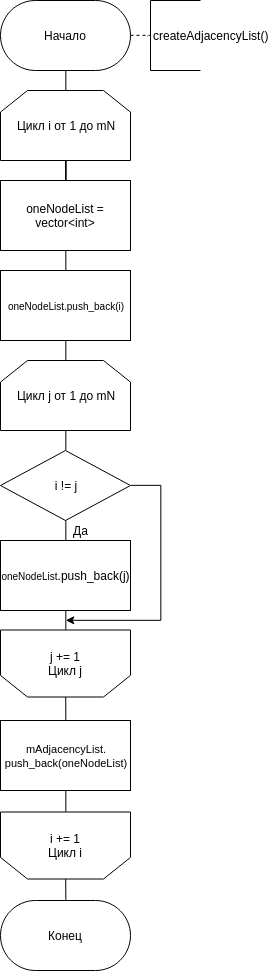
\includegraphics[height=20cm]{alist}}
\caption{Схема метода createAdjacencyList()}
\label{fig:image}
\end{figure}

\begin{figure}
\center{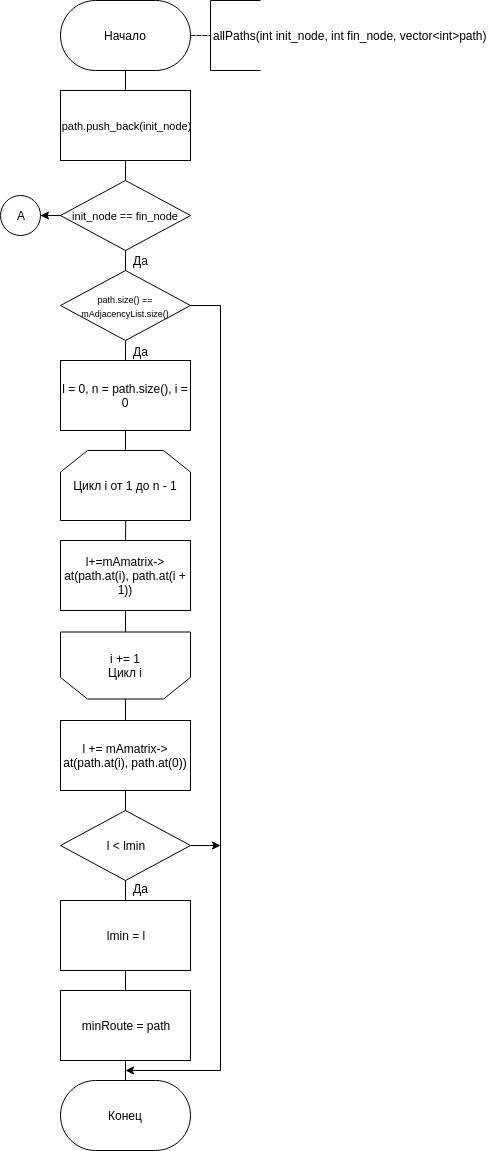
\includegraphics[height=20cm]{allp1}}
\caption{Схема метода allPaths()}
\label{fig:image}
\end{figure}

\begin{figure}
\center{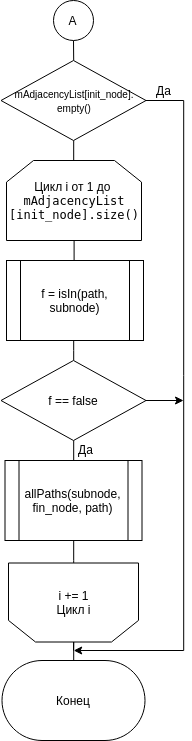
\includegraphics[height=20cm]{allp2}}
\caption{Схема метода allPaths() (продолжение)}
\label{fig:image}
\end{figure}

\begin{figure}
\center{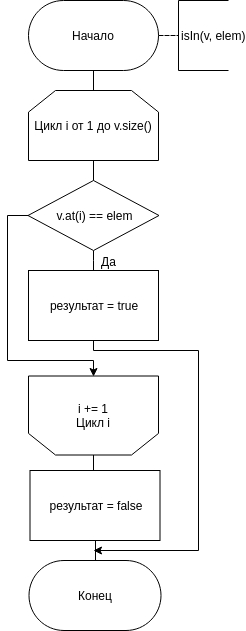
\includegraphics[height=20cm]{isin}}
\caption{Схема метода isIn()}
\label{fig:image}
\end{figure}

Приведем псевдокод муравьиного алгоритма для задачи коммивояжёра [1].

\begin{enumerate}
	\item Ввод матрицы расстояний D.
	\item Инициализация параметров алгоритма — $\alpha$, $\beta$, $\rho$, Q.
	\item Инициализация ребер — присвоение начальной концентрации феромона $\tau_{start}$.
	\item Размещение муравьев в случайно выбранные города.
	\item Выбор начального кратчайшего маршрута $T_{best}$ и определение его длины $L_{best}$.
	\item Цикл по времени жизни колонии $t=1,...,t_{max}$.
	\item Цикл по всем муравьям $k=1,...,m$
	\item Построить маршрут $T_{k}(t)$ по правилу (1) и рассчитать длину $L_{k}(t)$.
	\item Конец цикла по муравьям.
	\item Проверка всех $L_{k}(t)$ на лучшее решение по сравнению с $L_{best}$.
	\item Если да, то обновить  $L_{best}$ и  $T_{best}$.
	\item Цикл по всем ребрам графа.
	\item Обновить следы феромона на ребре по правилам (2) и (3).
	\item Конец цикла по ребрам.
	\item Конец цикла по времени.
	\item Вывести кратчайший маршрут $T_{best}$ и его длину $L_{best}$.
\end{enumerate}

Все формулы, необходимые для муравьиного алгоритма, были в аналитическом разделе.

\chapter*{Технологическая часть}
\addcontentsline{toc}{chapter}{Технологическая часть}

В данном разделе будут определены средства реализации и приведен листинг кода.

\section*{Выбор языка программирования}
\addcontentsline{toc}{section}{Выбор языка программирования}

В качестве языка программирования для реализации программы был выбран язык C++ и фреймворк Qt, потому что:
\begin{itemize}
	\item язык C++ имеет высокую вычислительную производительность;
	\item язык C++ поддерживает различные стили программирования;
	\item в Qt существует удобный инструмент для тестирования - QtTest - который позволяет собирать тесты в группы, собирать результаты выполнения тестов, а также уменьшить дублирование кода при схожих объектах тестирования.
\end{itemize}

Для замеров времени использовалась функция clock() модуля ctime. Эта функция возвращает количество временных тактов, прошедших с начала запуска программы.
С помощью макроса CLOCKS\_PER\_SEC можно узнать количество пройденных тактов за 1 секунду.

\section*{Сведения о модулях программы}
\addcontentsline{toc}{section}{Сведения о модулях программы}

Программа состоит из следующих файлов:
\begin{itemize}
	\item adjacencymatrix.h, adjacencymatrix.cpp - заголовочный файл и файл, в котором расположена реализация класса матрицы смежности;
	\item main.cpp - главный файл программы;
	\item algorithm.h, algorithm.cpp - файл и заголовочный файл, в котором расположена реализация класса Algorithm, который является родителем для классов BruteForce и AntColony;
	\item antcolony.h, antcolony.cpp - файл и заголовочный файл, в котором расположена реализация муравьиного алгоритма;
	\item bruteforce.h, bruteforce.cpp - файл и заголовочный файл, в котором расположена реализация алгоритма полгого перебора для задачи коммивояжёра;
	\item testsalesman.h, testsalesman.cpp - файл и заголовочный файл, в котором расположены тесты.
\end{itemize}

\section*{Листинги кода алгоритмов}
\addcontentsline{toc}{section}{Листинги кода алгоритмов}

В листинге 1 приведено объявление класса AntColony. В листинге 2 приведена реализация класса AntColony.

\begin{lstlisting}[label=some-code,caption=Объявление класса AntColony]
class AntColony : public Algorithm
{
public:
    AntColony();
    int getMinRoute(AdjacencyMatrix *amatrix, size_t alpha, size_t beta, double q, size_t tmax);
    vector<int> getMinRoute();
private:
    int lmin = INT_MAX;
    vector<int> minRoute;
    AdjacencyMatrix *mAmatrix;
    unsigned int mN;

    void getRoute(vector<int> all, int start, vector<int> &route, size_t &len,
                   vector<vector<double>> tao, vector<vector<double>> attraction,
                   size_t alpha, size_t beta);
    vector<int> deleteFromVector(vector<int> to, int last);
    vector<double> getProbability(int from, vector<int> to, vector<vector<double>> tao, vector<vector<double>> attraction,
                                   size_t alpha, size_t beta);
    bool includes(int a, int b, vector<int> route);
};
\end{lstlisting}

\begin{lstlisting}[label=some-code,caption=Реализация класса AntColony]
#include "antcolony.h"

AntColony::AntColony()
    : Algorithm ()
{

}

void AntColony::getRoute(vector<int> all, int start, vector<int> &route, size_t &len, vector<vector<double>> tao, vector<vector<double>> attraction, size_t alpha, size_t beta)
{
    route.resize(0);
    route.push_back(start);
    vector<int> to = deleteFromVector(all, start);
    size_t n_1 = tao.size() - 2;
    int from;
    double coin, sum;
    bool flag;

    for (size_t i = 0; i < n_1; i++){
        sum = 0;
        flag = true;
        from = route[i];
        vector<double> p = getProbability(from, to, tao, attraction, alpha, beta);
        coin = double(rand() % 10000) / 10000;
        for (size_t j = 0; j < p.size() && flag; j++)
				{
            sum += p[j];
            if (coin < sum)
						{
                route.push_back(to[j]);
                len += mAmatrix->at(from, to[j]);
                to = deleteFromVector(to, to[j]);
                flag = false;
            }
        }
    }
    len += mAmatrix->at(route[route.size()-1], to[0]);
    route.push_back(to[0]);
    len += mAmatrix->at(route[route.size()-1], route[0]);
    route.push_back(route[0]);
}

int AntColony::getMinRoute(AdjacencyMatrix *amatrix, size_t alpha, size_t beta, double q, size_t tmax)
{
    lmin = INT_MAX;
    minRoute.clear();

    this->mAmatrix = amatrix;
    this->mN = static_cast<unsigned int>(mAmatrix->cities());

    double tao_min, tao_start, Q;
    vector<int> all(mN);
    Q = 350;
    tao_min = 0.001;
    tao_start = 1.0 / mN;

    vector<vector<int>> routes(mN);
    vector<size_t> lens(mN);

    vector<vector<double>> attraction(mN);
    vector<vector<double>> tao(mN);

    for (size_t i = 0; i < mN; i++)
    {
        attraction[i].resize(mN);
        tao[i].resize(mN);
        lens[i] = 0;
        all[i] = static_cast<int>(i);
        for (size_t j = 0; j < mN; j++)
        {
            if (i != j)
						{
                attraction[i][j] = 1.0 / mAmatrix->at(i, j);
                tao[i][j] = tao_start;
            }
        }
    }

    for (size_t time = 0; time < tmax; time++)
		{
        for (size_t k = 0; k < mN; k++)
				{
            getRoute(all, static_cast<int>(k), routes[k], lens[k], tao, attraction, alpha, beta);
            if (lens[k] < lmin)
            {
                lmin = lens[k];
                minRoute = routes[k];
             }
        }
        for (size_t i = 0; i < mN; i++)
            for (size_t j = 0; j < mN; j++)
            {
                double sum = 0;
                for (size_t m = 0; m < mN; m++)
                {
                    if (includes(static_cast<int>(i), static_cast<int>(j), routes[m]))
                        sum += Q/lens[m];
                }

                tao[i][j] = tao[i][j]*(1 - q) + sum;
                if (tao[i][j] < tao_min)
                     tao[i][j] = tao_min;
            }
    }
    return lmin;
}

vector<int> AntColony::getMinRoute()
{
    return minRoute;
}

bool AntColony::includes(int a, int b, vector<int> route)
{
    bool res = false;
    size_t m = route.size()-1;
    for (size_t i = 0; i < m; i++)
		{
        if (a == route[i] && b == route[i+1])
            res = true;
    }
    return res;
}

vector<int> AntColony::deleteFromVector(vector<int> to, int last)
{
    size_t n = to.size();
    vector<int> cur;
    for (size_t i = 0; i < n; i++)
        if (to[i] != last)
            cur.push_back(to[i]);
    return cur;
}

vector<double> AntColony::getProbability(int from, vector<int> to,
                                         vector<vector<double>> tao, vector<vector<double>> attraction,
                                         size_t alpha, size_t beta)
{
    double znam = 0, chisl = 0;
    size_t n = to.size();
    vector<double> result(n);
    for (size_t i = 0; i < n; i++)
		{
        znam += pow(tao[from][to[i]], alpha) * pow(attraction[from][to[i]], beta);
    }
    for (size_t j = 0; j < n; j++)
		{
        chisl = pow(tao[from][to[j]], alpha) * pow(attraction[from][to[j]], beta);
        result[j] = chisl / znam;
    }
    return result;
}
\end{lstlisting}

\begin{lstlisting}[label=some-code,caption=Объявление класса BruteForce]
class BruteForce : public Algorithm
{
public:
    BruteForce();
    int getMinRoute(AdjacencyMatrix *amatrix);
    vector<int> getMinRouteVec();
private:
    void createAdjacencyList();
    void printVec(vector<int> &vec);
    bool isIn(vector<int> v, int elem);
    void allPaths(int init_node, int fin_node,
                  vector<int> path);

    int lmin = INT_MAX;
    vector<int> minRoute;
    AdjacencyMatrix *mAmatrix;
    vector<vector<int>> mAdjacencyList;
    int mN;
};
\end{lstlisting}

\begin{lstlisting}[label=some-code,caption=Реализация класса BruteForce]

#include "bruteforce.h"

BruteForce::BruteForce()
    : Algorithm ()
{

}


int BruteForce::getMinRoute(AdjacencyMatrix *amatrix)
{
    if (amatrix->cities() > 15)
        throw logic_error("Search will take too much time!\n");

    this->mAmatrix = amatrix;
    this->mN = mAmatrix->cities();
    minRoute.clear();

    createAdjacencyList();

    for (int i = 0; i < mN; ++i)
        for (int j = 0; j < mN; ++j)
        {
            if (i != j)
            {
                vector<int> b;
                allPaths(i, j, b);
            }
        }

//    printVec(minRoute);
//    cout << lmin << endl;

    return lmin;
}

void BruteForce::createAdjacencyList()
{
    for (int i = 0; i < mN; ++i)
    {
        vector<int> oneNodeList;
        oneNodeList.push_back(i);

        for (int j = 0; j < mN; ++j)
        {
            if (i != j)
                oneNodeList.push_back(j);
        }

        mAdjacencyList.push_back(oneNodeList);
    }
}

void BruteForce::allPaths(int init_node, int fin_node, vector<int>path)
{
    path.push_back(init_node);

    if (init_node == fin_node)
    {
        // path found
        if (path.size() == mAdjacencyList.size())
        {
            int l = 0, n = static_cast<int>(path.size()), i;
            for (i = 0; i < n - 1; ++i)
            {
                l += mAmatrix->at(path.at(i), path.at(i + 1));
            }
            l += mAmatrix->at(path.at(i), path.at(0));
            if (l < lmin)
            {
                lmin = l;
                minRoute = path;
            }
        }
        return;
    }

    if (mAdjacencyList[init_node].empty())
        return; // path not found

    for (auto subnode:mAdjacencyList[init_node])
    {
        if (!isIn(path, subnode))
            allPaths(subnode, fin_node, path);
    }
    return;
}

vector<int> BruteForce::getMinRouteVec()
{
    return minRoute;
}

void BruteForce::printVec(vector<int> &vec)
{
    for (unsigned int i = 0; i < vec.size(); ++i)
    {
        cout << vec.at(i) << "\t";
    }
    cout << endl;
}

bool BruteForce::isIn(vector<int>v, int elem)
{
    for (unsigned int i = 0; i < v.size(); ++i)
        if (v.at(i) == elem)
            return true;
    return false;
}
\end{lstlisting}

\section*{Тесты}
\addcontentsline{toc}{section}{Тесты}

Тестирование проводилось с помощью модуля QtTest. Для этого был написан класс TestSalesman. Сначала каждый алгоритм тестировался по отдельности на заранее заготовленном наборе тестовых данных .
После этого на матрицах смежности размерности 6 x 6 проводилось сравнение результата, полученного муравьиным алгоритмом, и результата, полученного в результате полного перебора.

В тестировании для муравьиного алгоритма использовались следующие параметры.

\begin{enumerate}
	\item $\alpha$ = 1.
	\item $\beta$ = 9.
	\item $\rho$ = 0.1.
	\item $t_{max}$ = 100.
	\item $\tau_{min}$ = 0.001.
	\item $\tau_{start}$ = $\frac{1}{количество городов}$.
	\item $Q$ = 350.
\end{enumerate}

Все написанные тесты были пройдены.

Использованный набор тестовых данных приведен в таблице 1 и в таблице 2.

\begin{table}[h]
	\caption{Набор тестовых данных}
	%\begin{center}
		\begin{tabular}{|c | c |}
	 	\hline
		Матрица смежности & Ожидаемый результат \\ [0.5ex]
	 	\hline\hline
		$\begin{bmatrix}
		0 & 1 \\
		1 & 0 \\
		\end{bmatrix}$ & 2 \\
		\hline

		$\begin{bmatrix}
		0 & 1 & 1 \\
		1 & 0 & 1 \\
		1 & 1 & 0 \\
		\end{bmatrix}$ & 3 \\
		\hline

		$\begin{bmatrix}
		0 & 3 & 1 \\
		3 & 0 & 2 \\
		1 & 2 & 0 \\
		\end{bmatrix}$ & 6 \\
		\hline

		$\begin{bmatrix}
		0 & 1 & 1 & 1 \\
		1 & 0 & 1 & 1 \\
		1 & 1 & 0 & 1 \\
		1 & 1 & 1 & 0 \\
		\end{bmatrix}$ & 4 \\
		\hline

		$\begin{bmatrix}
		0 & 2 & 1 & 1 \\
		2 & 0 & 1 & 1 \\
		1 & 1 & 0 & 2 \\
		1 & 1 & 2 & 0 \\
		\end{bmatrix}$ & 4 \\
		\hline

		$\begin{bmatrix}
		0 & 1 & 4 & 6 \\
		1 & 0 & 5 & 2 \\
		4 & 5 & 0 & 3 \\
		6 & 2 & 3 & 0 \\
		\end{bmatrix}$ & 10 \\
		\hline

		$\begin{bmatrix}
		0 & 4 & 4 & 1 \\
		4 & 0 & 1 & 2 \\
		4 & 1 & 0 & 4 \\
		1 & 2 & 4 & 0 \\
		\end{bmatrix}$ & 8 \\
		\hline

		$\begin{bmatrix}
		0 & 4 & 4 & 1 \\
		4 & 0 & 3 & 2 \\
		4 & 3 & 0 & 4 \\
		1 & 2 & 4 & 0 \\
		\end{bmatrix}$ & 10 \\
		\hline

		$\begin{bmatrix}
		0 & 1 & 1 & 1 & 1 \\
		1 & 0 & 1 & 1 & 1 \\
		1 & 1 & 0 & 1 & 1 \\
		1 & 1 & 1 & 0 & 1 \\
		1 & 1 & 1 & 1 & 0 \\
		\end{bmatrix}$ & 5 \\
		\hline

		$\begin{bmatrix}
		0 & 1 & 1 & 1 & 1 \\
		1 & 0 & 1 & 5 & 1 \\
		1 & 1 & 0 & 1 & 1 \\
		1 & 5 & 1 & 0 & 1 \\
		1 & 1 & 1 & 1 & 0 \\
		\end{bmatrix}$ & 5 \\
		\hline

	\end{tabular}
%\end{center}
\end{table}

\begin{table}[h]
	\caption{Набор тестовых данных (продолжение)}
	%\begin{center}
		\begin{tabular}{|c | c |}
	 	\hline
		Матрица смежности & Ожидаемый результат \\ [0.5ex]
	 	\hline\hline

		$\begin{bmatrix}
		0 & 1 & 1 & 1 & 1 \\
		1 & 0 & 1 & 5 & 1 \\
		1 & 1 & 0 & 5 & 1 \\
		1 & 5 & 5 & 0 & 1 \\
		1 & 1 & 1 & 1 & 0 \\
		\end{bmatrix}$ & 5 \\
		\hline

		$\begin{bmatrix}
		0 & 1 & 1 & 1 & 1 \\
		1 & 0 & 1 & 5 & 5 \\
		1 & 1 & 0 & 5 & 5 \\
		1 & 5 & 5 & 0 & 1 \\
		1 & 5 & 5 & 1 & 0 \\
		\end{bmatrix}$ & 9 \\
		\hline

		$\begin{bmatrix}
		0 & 1 & 1 & 1 & 1 & 1 \\
		1 & 0 & 2 & 1 & 1 & 1 \\
		1 & 2 & 0 & 2 & 1 & 1 \\
		1 & 1 & 2 & 0 & 1 & 1 \\
		1 & 1 & 1 & 1 & 0 & 1 \\
		1 & 1 & 1 & 1 & 1 & 1 \\
		\end{bmatrix}$ & 6 \\
		\hline

		$\begin{bmatrix}
		0 & 2 & 1 & 1 & 1 & 1 \\
		2 & 0 & 2 & 1 & 1 & 1 \\
		1 & 2 & 0 & 2 & 1 & 1 \\
		1 & 1 & 2 & 0 & 2 & 1 \\
		1 & 1 & 1 & 2 & 0 & 1 \\
		1 & 1 & 1 & 1 & 1 & 0 \\
		\end{bmatrix}$ & 6 \\
		\hline

		\end{tabular}
	%\end{center}
\end{table}

\chapter*{Экспериментальная часть}
\addcontentsline{toc}{chapter}{Экспериментальная часть}

В данном разделе будет проведена параметризация муравьиного алгоритма.

Были выбраны три матрицы смежности размером 10 x 10.

Первая матрица ($M_{1}$):

$\begin{bmatrix}
0 & 40 & 30 & 10 & 70 & 25 & 50 & 60 & 40 & 35 \\
40 & 0 & 70 & 90 & 40 & 50 & 80 & 50 & 45 & 40 \\
30 & 70 & 0 & 60 & 20 & 80 & 40 & 60 & 65 & 80 \\
10 & 90 & 60 & 0 & 50 & 10 & 80 & 15 & 90 & 30 \\
70 & 40 & 20 & 50 & 0 & 75 & 30 & 30 & 40 & 25 \\
25 & 50 & 80 & 10 & 75 & 0 & 10 & 20 & 10 & 70 \\
50 & 80 & 40 & 80 & 30 & 10 & 0 & 70 & 40 & 30 \\
60 & 50 & 60 & 15 & 30 & 20 & 70 & 0 & 20 & 80 \\
40 & 45 & 65 & 90 & 40 & 10 & 40 & 20 & 0 & 90 \\
35 & 40 & 80 & 30 & 25 & 70 & 30 & 80 & 90 & 0 \\
\end{bmatrix}$

Вторая матрица ($M_{2}$):

$\begin{bmatrix}
0 & 30 & 40 & 10 & 70 & 25 & 50 & 60 & 40 & 20 \\
30 & 0 & 70 & 90 & 40 & 50 & 80 & 50 & 45 & 40 \\
40 & 70 & 0 & 30 & 50 & 80 & 40 & 60 & 65 & 80 \\
10 & 90 & 30 & 0 & 50 & 10 & 80 & 15 & 90 & 30 \\
70 & 40 & 50 & 50 & 0 & 75 & 50 & 30 & 40 & 25 \\
25 & 50 & 80 & 10 & 75 & 0 & 5 & 20 & 10 & 70 \\
50 & 80 & 40 & 80 & 50 & 5 & 0 & 70 & 40 & 30 \\
60 & 50 & 60 & 15 & 30 & 20 & 70 & 0 & 20 & 80 \\
40 & 45 & 65 & 90 & 40 & 10 & 40 & 20 & 0 & 75 \\
20 & 40 & 80 & 30 & 25 & 70 & 30 & 80 & 75 & 0 \\
\end{bmatrix}$

Третья матрица ($M_{3}$):

$\begin{bmatrix}
%0 & 10 & 10 & 10 & 30 & 25 & 34 & 60 & 44 & 21 \\
%10 & 0 & 70 & 90 & 40 & 50 & 80 & 50 & 45 & 77 \\
%10 & 70 & 0 & 32 & 50 & 80 & 40 & 60 & 65 & 88 \\
%10 & 90 & 32 & 0 & 53 & 10 & 80 & 15 & 59 & 33 \\
%30 & 40 & 50 & 53 & 0 & 71 & 10 & 32 & 40 & 25 \\
%25 & 50 & 80 & 10 & 71 & 0 & 5 & 20 & 10 & 70 \\
%34 & 80 & 40 & 80 & 10 & 5 & 0 & 23 & 40 & 16 \\
%60 & 50 & 60 & 15 & 32 & 20 & 23 & 0 & 27 & 47 \\
%44 & 45 & 65 & 59 & 40 & 10 & 40 & 27 & 0 & 75 \\
%21 & 77 & 88 & 33 & 25 & 70 & 16 & 47 & 75 & 0 \\
0 & 30 & 30 & 20 & 70 & 25 & 50 & 60 & 40 & 30 \\
30 & 0 & 70 & 90 & 40 & 50 & 80 & 50 & 45 & 40 \\
30 & 70 & 0 & 50 & 25 & 80 & 40 & 60 & 65 & 40 \\
20 & 90 & 50 & 0 & 40 & 10 & 80 & 15 & 90 & 35 \\
70 & 40 & 25 & 40 & 0 & 75 & 30 & 30 & 40 & 25 \\
25 & 50 & 80 & 10 & 75 & 0 & 10 & 20 & 10 & 60 \\
50 & 80 & 40 & 80 & 30 & 10 & 0 & 70 & 40 & 30 \\
60 & 50 & 60 & 15 & 30 & 20 & 70 & 0 & 20 & 70 \\
40 & 45 & 65 & 90 & 40 & 10 & 40 & 20 & 0 & 80 \\
30 & 40 & 40 & 35 & 25 & 60 & 30 & 70 & 80 & 0 \\
\end{bmatrix}$

\section*{Постановка эксперимента}
\addcontentsline{toc}{section}{Постановка эксперимента}

В рамках данной работы были проведены следующие эксперименты.

\begin{enumerate}
	\item Для различных значений параметров $\alpha$, $\beta$, $\rho$ и $t_{max}$ для кадой из трех матриц смежности $M_{1}$, $M_{2}$ и $M_{3}$ с помощью муравьиного алгоритма была найдена некоторая длина маршрута.
 	\item С помощью перебора был найен самый короткий маршрут для кадой из трех матриц смежности $M_{1}$, $M_{2}$ и $M_{3}$.
	\item Было проведено сравнение длины маршута, полученной с помощью муравьиного алгоритма и с помощью полного перебора.
	\item На основании сравнения были выбраны наилучшие сочетания параметров муравьиного алгоритма на данном классе данных.
\end{enumerate}

Значения параметров изменялись в следующих диапазонах.

\begin{enumerate}
	\item $\alpha$ $\in$ $\{0, 1, 2, 3, 4, 5, 6, 7, 8, 9, 10\}$.
	\item $\beta$ + $\alpha$ = const.
	\item $\rho$ $\in$ $\{0.1, 0.2, 0.25, 0.3, 0.4, 0.5, 0.6, 0.7, 0.75, 0.8, 0.9\}$.
	\item $t_{max}$ $\in$ $\{5, 10, 20, 30, 40, 50, 60, 70, 80, 90, 100\}$.
\end{enumerate}

Измерения проводились на компьютере HP Pavilion Notebook на базе Intel Core i5-7200U, 2.50 Гц с 6 Гб оперативной памяти и с 4 логическими ядрами под управлением операционной системы Linux Mint.

\section*{Параметризация муравьиного алгоритма на основании проведенного эксперимента}
\addcontentsline{toc}{section}{Сравнительный анализ на материале экспериментальных данных}

В таблице 3 приведены сочетания параметров, при которых муравьный алгоритм давал наиболее оптимальное решение для всех трех матриц.
Условные обозначения в таблице 3:
\begin{enumerate}
	\item B1 - длина маршрута для матрицы $M_{1}$, рассчитанная с помощью полгого перебора;
	\item A1 - длина маршрута для матрицы $M_{1}$, рассчитанная с помощью муравьиного алгоритма;
	\item B2 - длина маршрута для матрицы $M_{2}$, рассчитанная с помощью полгого перебора;
	\item A2 - длина маршрута для матрицы $M_{2}$, рассчитанная с помощью муравьиного алгоритма;;
	\item B3 - длина маршрута для матрицы $M_{3}$, рассчитанная с помощью полгого перебора;
	\item A3 - длина маршрута для матрицы $M_{4}$, рассчитанная с помощью муравьиного алгоритма;.
\end{enumerate}


\begin{table}[h]
	\caption{Наиболее оптимальные сочетания параметров}
	%\begin{center}
		\begin{tabular}{| c | c | c | c || c | c || c | c || c | c |}
	 	\hline
		$\alpha$ & $\beta$ & $\rho$ & $t_{max}$ & B1 & A1 & B2 & A2 & B3 & A3 \\ [0.5ex]
	 	\hline\hline
		4 & 6 & 0.6 & 20 & 225 & 225 & 240 & 240 & 235 & 240 \\ \hline
		6 & 4 & 0.3 & 40 & 225 & 225 & 240 & 245 & 235 & 240 \\ \hline
		1 & 9 & 0.7 & 50 & 225 & 225 & 240 & 245 & 235 & 240 \\ \hline
		6 & 4 & 0.9 & 70 & 225 & 230 & 240 & 245 & 235 & 240 \\ \hline
		3 & 7 & 0.6 & 80 & 225 & 230 & 240 & 245 & 235 & 240 \\ \hline
		6 & 4 & 0.25 & 90 & 225 & 230 & 240 & 240 & 235 & 235 \\ \hline
		\end{tabular}
	%\end{center}
\end{table}

\section*{Выводы}
\addcontentsline{toc}{section}{Выводы}

Таким образом, для заданного класса данных были найдены параметры, которые обеспечивают наиболее оптимальное решение.

\chapter*{Заключение}
\addcontentsline{toc}{chapter}{Заключение}

Таким образом, в ходе выполнения данной лабораторной работы был приобретен навык параметризации метода на примере решения задачи коммивояжёра методом, основанным на муравьином алгоритме. Был произведен отбор таких сочетаний параметров, при котором муравьиный алгоритм решает заданный класс задач наилучшим образом. Таким образом была минимизирована разница между муравьиным алгоритмом и полным перебором.

\chapter*{Список литературы}
\addcontentsline{toc}{chapter}{Список литературы}

1. Ульянов М. В. Ресурсно-эффективные компьютерные алгоритмы. Разработка и анализ. -М.:Наука, 2007.

\end{document}
